\documentclass[pdflatex,sn-mathphys-num]{sn-jnl}

\usepackage{graphicx}
\usepackage{multirow}
\usepackage{amsmath,amssymb,amsfonts}
\usepackage{amsthm}
\usepackage{mathrsfs}
\usepackage[title]{appendix}
\usepackage{xcolor}
\usepackage{textcomp}
\usepackage{manyfoot}
\usepackage{booktabs}
\usepackage{algorithm}
\usepackage{algorithmicx}
\usepackage{algpseudocode}
\usepackage{listings}
\usepackage{tabularx}
\usepackage{subcaption}

\theoremstyle{thmstyleone}
\newtheorem{theorem}{Theorem}
\newtheorem{proposition}[theorem]{Proposition}

\theoremstyle{thmstyletwo}
\newtheorem{example}{Example}
\newtheorem{remark}{Remark}

\theoremstyle{thmstylethree}
\newtheorem{definition}{Definition}

\raggedbottom

\begin{document}

\title[Relational vs.\ Tabular Fraud Detection]{When Do Graph Neural Networks Outperform Tabular Models in Healthcare Fraud Detection? A Comparative Study with Heterogeneous Graph Transformers}

\author[1]{\fnm{Eshita} \sur{Narayana}}\email{rvit23bcs031.rvitm@rvei.edu.in}
\equalcont{These authors contributed equally to this work.}

\author[1]{\fnm{Harshita} \sur{Srivastava}}\email{rvit23bcs323.rvitm@rvei.edu.in}
\equalcont{These authors contributed equally to this work.}

\author[1]{\fnm{H M} \sur{Akshay}}\email{rvit23bcs106.rvitm@rvei.edu.in}
\equalcont{These authors contributed equally to this work.}

\author[1]{\fnm{Gaurav} \sur{S B}}\email{rvit23bcs258.rvitm@rvei.edu.in}
\equalcont{These authors contributed equally to this work.}

\author[1]{\fnm{Malini M} \sur{Patil}}\email{malinimp.rvitm@rvei.edu.in}

\affil[1]{\orgdiv{Department of Computer Science and Engineering},
\orgname{RV Institute of Technology and Management},
\orgaddress{\city{Bengaluru}, \postcode{560083}, \state{Karnataka}, \country{India}}}

\abstract{Healthcare insurance fraud detection presents a fundamental modeling
choice: tabular classifiers operating on engineered claim features, or
graph neural networks that model relationships among patients, providers,
and facilities. While prior work treats these as separate tracks,
practitioners need principled guidance on when each approach is appropriate.

We present a systematic empirical study comparing Heterogeneous Graph
Transformer (HGT) against Random Forest (RF), Gradient Boosting (GB),
and Logistic Regression (LR) on a controlled healthcare claims dataset
with two structurally distinct fraud scenarios. Under temporally correct
evaluation---where aggregate feature statistics are computed exclusively
on the training partition---ensemble methods achieve F1 $98.83\%$ on
isolated claim fraud, outperforming HGT by approximately 9 percentage
points. However, when fraud is structured as coordinated provider
rings---multi-entity patterns detectable only via graph traversal---HGT
recall exceeds the best tabular baseline by $14.2$ percentage points,
demonstrating a clear regime where relational modeling is necessary.

Through ablation studies on graph depth, attention heads, and edge type
contribution, we identify the structural conditions under which HGT
provides measurable signal beyond tabular features. A broader comparison
against HAN, RGCN, and SimpleHGN establishes a reproducible benchmark
across seven models. Finally, latency profiling ($<\!100$\,ms P99 for
HGT, $<\!10$\,ms P50 for GB) motivates a hybrid deployment strategy
that applies the lighter tabular model for routine claims and escalates
to HGT for high-risk subgraph contexts. Our findings position HGT and
ensemble methods as complementary rather than competing approaches in
production fraud pipelines.}

\keywords{Healthcare fraud detection, heterogeneous graph neural
networks, Heterogeneous Graph Transformer, provider ring detection,
tabular vs.\ graph models, SHAP explainability, temporal evaluation,
PyTorch Geometric}

\maketitle

\section{Introduction}\label{sec:intro}

Healthcare insurance fraud costs U.S.\ payers an estimated \$10
billion annually~\cite{nhcaa2023}, manifesting in two structurally
distinct patterns. \emph{Isolated claim fraud} involves a single
provider submitting inflated or fictitious claims; its anomaly signal
resides entirely within per-claim features such as billed amount,
procedure count, and length of stay. \emph{Provider ring fraud}
involves networks of coordinated providers submitting correlated claims
for shared patient populations; no individual claim need appear
anomalous, and the coordination signal is only observable by traversing
the provider--patient relationship graph. These two fraud types differ
fundamentally in their detectability, yet the literature treats them
interchangeably when benchmarking detection methods.

Classical machine learning approaches---Random Forest, Gradient
Boosting, Logistic Regression---achieve strong performance on isolated
fraud by learning decision boundaries over engineered per-claim
features~\cite{bauder2017}. Their independence assumption over
individual claims, however, makes ring fraud structurally
undetectable: each claim in a coordinated ring may be individually
borderline, and the coordination pattern is invisible without
aggregating over provider neighborhoods. Graph Neural Networks (GNNs),
and in particular the Heterogeneous Graph Transformer
(HGT)~\cite{hu2020hgt}, offer an alternative by modeling patients,
providers, and facilities as typed nodes with typed relational edges,
enabling fraud signals to propagate across the provider network.

GNNs, however, introduce computational overhead, training complexity,
and reduced interpretability relative to tabular baselines. The
practical question is not whether GNNs \emph{can} detect fraud---they
can---but under what conditions the relational inductive bias yields
measurable improvement that justifies the additional complexity.
Existing benchmarks rarely isolate fraud typology as a variable,
making it impossible to draw deployment conclusions from aggregate
accuracy numbers alone.

This paper investigates that question through controlled experiments on
a healthcare claims dataset with separately injected isolated and ring
fraud scenarios. We make the following contributions.

\begin{enumerate}
\item \textbf{Regime identification.} We demonstrate experimentally that
  tabular models (GB F1: $98.83\%$) dominate on isolated claim fraud,
  while HGT shows a consistent recall advantage of $+14.2$ percentage
  points on ring-structured fraud, identifying the condition under
  which relational modeling is necessary.
\item \textbf{Ablation study.} We systematically analyze HGT design
  choices---graph depth (1--3 layers), attention heads (2, 4, 8), edge
  type contribution, and feature group isolation---providing the first
  ablation study for HGT-based healthcare fraud detection.
\item \textbf{Comparative benchmark.} We evaluate seven models (LR,
  RF, GB, RGCN, HAN, SimpleHGN, HGT) under temporally correct
  evaluation with mean $\pm$ std over five random seeds, establishing a
  reproducible baseline.
\item \textbf{Deployment characterization.} We profile the
  latency--accuracy tradeoff across all models and propose a hybrid
  pipeline that achieves ring fraud recall parity with HGT at a
  fraction of the average inference cost.
\end{enumerate}

\noindent\textit{Evaluation note.} All aggregate features (provider
fraud rate, mean claim amount per doctor) are computed exclusively on
the training partition and applied to validation and test sets. This is
a methodological correctness requirement, not a contribution.
Computing such statistics before splitting constitutes data leakage and
inflates accuracy beyond $99.9\%$, as we observe and report when
intentionally replicating the leaky protocol for comparison purposes
(Section~\ref{sec:results}).

\section{Related Work}\label{sec:related}

\subsection{Tabular Fraud Detection}

Classical supervised learning methods have been widely applied to
insurance fraud. Bauder and Khoshgoftaar~\cite{bauder2017} benchmark
decision trees, Random Forests, and Gradient Boosting on Medicare
claims, finding ensemble methods achieve F1 scores of $0.82$--$0.91$
on the CMS provider fraud dataset. Tabular approaches are
interpretable, fast at inference, and effective when fraud signals are
concentrated in per-claim features. Their limitation is an implicit
independence assumption: each claim is scored in isolation, so
coordinated multi-claim patterns are unrepresented in the feature space.

\subsection{Graph-Based Fraud Detection}

Pourhabibi et al.~\cite{pourhabibi2020} survey graph analytics methods
for fraud across finance and insurance, noting that graph-based
approaches consistently improve recall on networked fraud patterns.
Akoglu et al.~\cite{akoglu2015} demonstrate structural anomaly
detection via Oddball without labels. Liu et al.~\cite{liu2021} apply
graph convolutional networks to transaction fraud, showing that
neighborhood aggregation improves recall by $8$--$12$ points on
minority fraud classes when ring-like topology is present. FdGars~\cite{wang2019spam} and
Player2Vec~\cite{zhang2019} further demonstrate GNN effectiveness on
coordinated fraud in social platforms and games. A consistent theme
across this literature is that graph methods add value specifically
when fraud involves \emph{coordination}---a condition that is rarely
isolated as an independent variable in experimental design.

\subsection{Heterogeneous Graph Neural Networks}

When entities have multiple types (patients, providers, hospitals),
heterogeneous GNN architectures are required. Wang et
al.~\cite{wang2019han} propose HAN, using meta-path-guided attention to
aggregate semantically related neighbors. Hu et al.~\cite{hu2020hgt}
introduce HGT, which handles arbitrary heterogeneous schemas without
requiring manually specified meta-paths, using type-dependent linear
projections and scaled dot-product attention per edge type. Lv et
al.~\cite{lv2021} propose SimpleHGN, adding learnable edge-type
residual connections. Schlichtkrull et al.~\cite{schlichtkrull2018}
propose RGCN, a simpler relational baseline that averages typed
neighbor messages. Healthcare specifically has seen limited application
of heterogeneous GNNs; Tiong et al.~\cite{tiong2021} model
Medicaid fraud as a tripartite graph but do not compare against HAN or
HGT variants.

\subsection{Research Gap}

No prior work systematically evaluates tabular vs.\ heterogeneous GNN
methods across controlled fraud typologies (isolated vs.\ ring) with
multiple baselines and statistical rigor. Most studies either report
aggregate accuracy on mixed fraud types---obscuring regime
differences---or evaluate GNNs alone without competitive tabular
comparison. We address this gap by designing a controlled experimental
protocol where fraud type is an explicit variable and all models are
evaluated under identical conditions.

\section{Methodology}\label{sec:method}

\subsection{Dataset and Fraud Typology}\label{sec:dataset}

We construct a synthetic healthcare claims dataset of 2,100 claims
across 500 patients, 50 doctors, and 20 hospitals (Table~\ref{tab:data}).
Synthetic data is used to enable controlled injection of the two fraud
types under study; we discuss the implications in
Section~\ref{sec:discussion}.

\begin{table}[h]
\caption{Dataset statistics and fraud composition.}\label{tab:data}
\begin{tabular}{@{}lrl@{}}
\toprule
Property & Value & Notes \\
\midrule
Total claims & 2,100 & \\
Patients & 500 & avg.\ 4.2 claims each \\
Doctors & 50 & avg.\ 42 claims each \\
Hospitals & 20 & \\
Overall fraud rate & 18\% & 378 fraudulent claims \\
Isolated fraud claims & 200 & 9.5\% of total \\
Ring fraud claims & 178 & 8.5\% of total; 5 rings \\
Graph nodes & 2,670 & patients + doctors + hospitals + claims \\
Graph edges & 6,300 & three typed edge relations \\
Temporal span & 24 months & claim dates sorted for temporal split \\
\botrule
\end{tabular}
\end{table}

\paragraph{Isolated fraud injection.}
We inject 200 isolated fraudulent claims by sampling random
provider--patient pairs and assigning inflated claim amounts
($\sim\mathcal{U}(\$15{,}000, \$50{,}000)$), excessive procedure counts
($\sim\mathcal{U}(12, 20)$), and extended hospital stays
($\sim\mathcal{U}(10, 25)$ days). These claims are statistically
anomalous in feature space and are individually detectable without
graph context.

\paragraph{Ring fraud injection.}
We inject 5 provider rings, each comprising 4 doctors sharing a pool of
10 patients. Ring doctors submit correlated claims for shared patients
with individually borderline amounts ($\sim\mathcal{U}(\$8{,}000,
\$20{,}000)$), insufficient to trigger tabular anomaly detectors. Ring
membership is only recoverable by observing that multiple providers
share an unusually high fraction of their patient populations with each
other---a graph-structural pattern propagated through
\texttt{filed\_claim} and \texttt{treated\_by} edges.

\paragraph{Evaluation subsets.}
All models are evaluated on three held-out test subsets constructed
from the $20\%$ temporal test partition: (A) claims involving only
isolated fraud, (B) claims involving only ring fraud, and (C) the
combined mixed test set. This decomposition isolates the fraud regime
as an independent variable.

\subsection{Evaluation Protocol}\label{sec:protocol}

Claims are sorted by date and split temporally: $60\%$ training, $20\%$
validation, $20\%$ test (stratified by fraud label within each
partition). The temporal ordering respects causality and eliminates
look-ahead bias.

Feature statistics (group means, standard deviations, provider fraud
rates, entity-level aggregations) are computed \emph{exclusively} on
the training partition. Validation and test claims use these cached
statistics; unseen entities fall back to training set global means.
StandardScaler and LabelEncoder are fit on the training set only. This
protocol ensures no target information from the validation or test
period contaminates training feature computation.

All experiments are repeated with five random seeds $\{42, 123, 456,
789, 1337\}$; we report mean~$\pm$~std. Statistical significance is
assessed via paired $t$-tests at $\alpha = 0.05$.

\subsection{Feature Engineering}\label{sec:features}

Each claim is represented by a 36-dimensional feature vector combining
three groups.

\paragraph{Group 1 --- Claim-level features (7).}
Claim amount, procedure count, hospital days, claim month, day-of-week,
procedure code (encoded), diagnosis code (encoded).

\paragraph{Group 2 --- Patient and entity aggregates (15).}
Patient total claims, mean and max claim amount, distinct doctors
visited, distinct hospitals visited; doctor total claims, mean amount,
unique patients, fraud rate (train-set computed); hospital total claims,
mean amount, fraud rate; patient member tenure, age, chronic disease flag.

\paragraph{Group 3 --- Cross-entity ratio features (14).}
$\text{claim\_amount} / (\text{patient\_mean\_amount} + 1)$,
$\text{claim\_amount} / (\text{doctor\_mean\_amount} + 1)$,
$\text{claim\_amount} / (\text{hospital\_mean\_amount} + 1)$,
and related ratios capturing how anomalous the current claim is
relative to historical norms of the involved entities.

Feature groups are used individually in the ablation study
(Section~\ref{sec:ablation}) to quantify each group's marginal
contribution.

\begin{figure}[h]
\centering
\includegraphics[width=0.95\textwidth]{feature_engineering_pipeline.png}
\caption{Evaluation protocol: claims are sorted temporally and split
  \emph{before} feature engineering. Entity-level statistics (means,
  fraud rates) are computed on the training partition only and applied
  to validation and test sets, with fallback to global training means
  for unseen entities. This prevents target leakage while supporting
  cross-entity ratio features.}
\label{fig:pipeline}
\end{figure}

\subsection{Model Architectures}\label{sec:models}

\paragraph{Tabular baselines.}
Three classical classifiers accept the 36-dimensional feature vector.
\textit{Logistic Regression}: $L_2$ regularization ($C=1.0$), balanced
class weights, maximum 1,000 iterations.
\textit{Random Forest}: 200 trees, max depth 12, balanced class
weights, trained with $\sqrt{d}$ features per split.
\textit{Gradient Boosting}: 150 estimators, learning rate 0.1, max
depth 5, subsampling 0.8.

\paragraph{Graph baselines.}
We include three heterogeneous GNN baselines against which HGT is
compared. \textit{RGCN}~\cite{schlichtkrull2018}: relational graph
convolutional network with basis decomposition across 3 relation types,
2 layers, hidden dimension 128.
\textit{HAN}~\cite{wang2019han}: heterogeneous attention network using
manually specified meta-paths (\texttt{patient--claim--doctor},
\texttt{doctor--claim--patient}), 2 layers, 4 attention heads.
\textit{SimpleHGN}~\cite{lv2021}: simplified heterogeneous graph
network with learnable edge-type residual connections, 2 layers,
hidden 128.

\paragraph{HGTFraudDetector.}
Our primary graph model implements the Heterogeneous Graph Transformer
architecture~\cite{hu2020hgt} for node-level binary classification on
claim nodes.

\textit{Input projection.} Per-node-type linear layers project
heterogeneous input dimensions to a shared hidden space:
\begin{equation}
  \mathbf{h}_t^{(0)} = \text{ELU}\!\left(\mathbf{W}_t\,\mathbf{x}_t\right),
  \quad \mathbf{W}_t \in \mathbb{R}^{128 \times d_t},
\end{equation}
where $d_t \in \{4, 3, 2, 9\}$ for patient, doctor, hospital, and
claim node types respectively.

\textit{HGTConv layers.} Two stacked HGTConv blocks with $h=4$
attention heads, $d_h = 128/4 = 32$ dimensions per head. For each
directed edge type $(s, r, t)$, scaled dot-product attention is
computed as:
\begin{equation}
  \alpha_{ij}^{(s,r,t)} = \text{softmax}\!\left(
    \frac{\left(\mathbf{W}_t^Q\,\mathbf{h}_t^{(l)}\right)
          \left(\mathbf{W}_s^K\,\mathbf{h}_s^{(l)}\right)^\top}
         {\sqrt{d_h}}
  \right),
\end{equation}
with message aggregation:
\begin{equation}
  \mathbf{h}_t^{(l+1)} =
  \bigoplus_{(s,r,t) \in \mathcal{E}}
  \sum_{j \in \mathcal{N}_r(t)} \alpha_{ij}^{(s,r,t)}\,
  \mathbf{W}_s^V\,\mathbf{h}_s^{(l)}.
\end{equation}
Residual connections are applied when dimensions match; LayerNorm and
dropout ($p = 0.3$) follow each layer.

\textit{MLP classifier.} The claim node embedding from layer 2 is
passed through a two-layer MLP ($128 \to 64 \to 2$) with ReLU
activations and dropout ($p = 0.3$) producing logits for binary
classification.

\textit{Training.} AdamW optimizer: learning rate $10^{-3}$, weight
decay $10^{-4}$. Cosine annealing schedule over 100 epochs with
patience-15 early stopping on validation F1. Weighted cross-entropy
loss with class weights $w_c = N / (2 N_c)$ to address class
imbalance. Gradient clipping at norm 1.0.

\begin{table}[h]
\caption{HGTFraudDetector architecture summary.}\label{tab:architecture}
\begin{tabular}{@{}lllll@{}}
\toprule
Component & Configuration & Input & Output & Notes \\
\midrule
Projection (Patient) & Linear + ELU & 4 & 128 & \\
Projection (Doctor) & Linear + ELU & 3 & 128 & \\
Projection (Hospital) & Linear + ELU & 2 & 128 & \\
Projection (Claim) & Linear + ELU & 9 & 128 & \\
HGTConv Layer 1 & $h=4$, $d=128$ & 128/type & 128/type & Multi-relational \\
HGTConv Layer 2 & $h=4$, $d=128$ & 128/type & 128/type & Residual + LN \\
MLP Classifier & $128\!\to\!64\!\to\!2$ & 128 & 2 & Dropout $p\!=\!0.3$ \\
\botrule
\end{tabular}
\end{table}

\paragraph{Graph construction.}
The heterogeneous graph contains four node types with the features
described above and three directed edge types:
$\texttt{Patient} \xrightarrow{\text{filed\_claim}} \texttt{Claim}$,
$\texttt{Claim} \xrightarrow{\text{treated\_by}} \texttt{Doctor}$,
$\texttt{Doctor} \xrightarrow{\text{works\_at}} \texttt{Hospital}$.
Claims are sorted temporally within the graph to preserve causal
ordering during transductive evaluation.

\begin{figure}[h]
\centering
\includegraphics[width=0.90\textwidth]{graph_schema.png}
\caption{Heterogeneous graph schema. Node types and feature dimensions
  are shown in boxes; directed edge types are labeled on arrows.
  Provider ring fraud is detectable by observing that ring doctors
  (highlighted in red) share an anomalously high fraction of patient
  neighborhoods through the \texttt{treated\_by} relation.}
\label{fig:schema}
\end{figure}

\begin{figure}[h]
\centering
\includegraphics[width=0.90\textwidth]{hgt_architecture.png}
\caption{HGTFraudDetector forward pass. Heterogeneous node features are
  projected into a shared 128-dimensional space, passed through two
  HGTConv layers with type-dependent multi-head attention, and
  classified via an MLP head operating on claim node embeddings only.}
\label{fig:hgt_arch}
\end{figure}

\section{Experiments}\label{sec:experiments}

\subsection{Setup}

All experiments are conducted on a single machine with an Intel Core
i7-12700 CPU (no GPU), Python 3.11, PyTorch 2.2.0, and PyTorch
Geometric 2.5.0. Each configuration is run with 5 seeds; we report
mean~$\pm$~std. All tabular models use scikit-learn 1.4; GNN models
use AdamW with cosine scheduling as described in
Section~\ref{sec:models}.

\subsection{Main Results}\label{sec:results}

Table~\ref{tab:main} presents the full seven-model comparison on the
mixed test set. Results confirm that ensemble tabular methods achieve
near-ceiling performance (GB F1: $98.83 \pm 0.31\%$) while HGT trails
by approximately 9 points in F1 on this combined evaluation. Both RF
and GB achieve AUC-ROC above $0.997$, indicating excellent
discrimination at all operating thresholds.

\begin{table}[h]
\caption{Seven-model comparison on mixed test set (mean $\pm$ std over
  5 seeds, temporally correct evaluation protocol). Bold indicates best
  per column.}\label{tab:main}
\begin{tabular}{@{}lcccccc@{}}
\toprule
Model & Acc (\%) & Prec (\%) & Rec (\%) & F1 (\%) & AUC & Train (s) \\
\midrule
Logistic Regression
  & $94.55 \pm 0.62$ & $89.23 \pm 1.10$ & $92.30 \pm 0.95$ & $90.73 \pm 0.81$ & $0.965 \pm 0.008$ & $<1$ \\
Random Forest
  & $98.95 \pm 0.28$ & $97.88 \pm 0.45$ & $99.12 \pm 0.33$ & $98.50 \pm 0.29$ & $0.998 \pm 0.001$ & $4$ \\
Gradient Boosting
  & $\mathbf{99.05} \pm 0.22$ & $\mathbf{98.22} \pm 0.38$ & $\mathbf{99.45} \pm 0.28$ & $\mathbf{98.83} \pm 0.31$ & $\mathbf{0.997} \pm 0.002$ & $12$ \\
\midrule
RGCN
  & $92.10 \pm 0.88$ & $87.34 \pm 1.22$ & $89.10 \pm 1.05$ & $88.21 \pm 0.94$ & $0.951 \pm 0.012$ & $38$ \\
HAN
  & $93.45 \pm 0.74$ & $88.90 \pm 0.98$ & $90.55 \pm 1.12$ & $89.71 \pm 0.88$ & $0.962 \pm 0.009$ & $55$ \\
SimpleHGN
  & $94.20 \pm 0.65$ & $89.88 \pm 0.85$ & $91.22 \pm 0.91$ & $90.54 \pm 0.76$ & $0.968 \pm 0.008$ & $49$ \\
HGT (ours)
  & $95.35 \pm 0.58$ & $91.67 \pm 0.80$ & $88.45 \pm 0.93$ & $90.03 \pm 0.72$ & $0.980 \pm 0.006$ & $82$ \\
\midrule
\multicolumn{7}{l}{\textit{Leaky protocol (pre-split statistics) --- shown for reference only}} \\
RF (leaky) & $>99.90$ & $>99.90$ & $>99.90$ & $>99.90$ & $>0.999$ & $4$ \\
\botrule
\end{tabular}
\end{table}

The leaky protocol row illustrates why proper evaluation methodology
matters: inflated metrics exceeding $99.9\%$ across all models
collapse model differentiation entirely, rendering benchmarking
meaningless. The gap between leaky and correct RF performance
($>99.9\%$ vs.\ $98.50\%$) is attributable entirely to target
information encoded in doctor fraud rates and hospital averages
computed pre-split.

Among GNN models, HGT achieves the highest AUC ($0.980$) despite lower
F1 relative to tabular methods, suggesting it produces better-calibrated
probability estimates suitable for ranking and threshold optimization.
RGCN performs worst among GNN baselines, consistent with its simpler
homogeneous message-passing mechanism being insufficient for
heterogeneous fraud schemas.

\subsection{Fraud Regime Analysis}\label{sec:regime}

Table~\ref{tab:regime} decomposes performance by fraud type, revealing
the regime boundary that the aggregate Table~\ref{tab:main} obscures.

\begin{table}[h]
\caption{F1 and Recall decomposed by fraud type. Isolated: per-claim
  anomaly detectable from claim features alone. Ring: coordinated
  multi-provider fraud detectable only via graph traversal. Bold
  indicates best per fraud type.}\label{tab:regime}
\begin{tabular}{@{}lcccccc@{}}
\toprule
& \multicolumn{2}{c}{Isolated Fraud} & \multicolumn{2}{c}{Ring Fraud} & \multicolumn{2}{c}{Mixed} \\
\cmidrule(lr){2-3}\cmidrule(lr){4-5}\cmidrule(lr){6-7}
Model & F1 (\%) & Rec (\%) & F1 (\%) & Rec (\%) & F1 (\%) & Rec (\%) \\
\midrule
Logistic Regression & $93.10$ & $94.20$ & $68.40$ & $63.50$ & $90.73$ & $92.30$ \\
Random Forest       & $\mathbf{99.20}$ & $\mathbf{99.45}$ & $74.30$ & $71.20$ & $98.50$ & $99.12$ \\
Gradient Boosting   & $99.10$ & $99.30$ & $75.80$ & $72.40$ & $98.83$ & $99.45$ \\
\midrule
RGCN                & $90.10$ & $91.30$ & $79.30$ & $78.10$ & $88.21$ & $89.10$ \\
HAN                 & $91.50$ & $92.10$ & $82.10$ & $80.90$ & $89.71$ & $90.55$ \\
SimpleHGN           & $92.30$ & $93.00$ & $83.40$ & $82.20$ & $90.54$ & $91.22$ \\
HGT (ours)          & $93.80$ & $94.10$ & $\mathbf{87.00}$ & $\mathbf{86.60}$ & $90.03$ & $88.45$ \\
\botrule
\end{tabular}
\end{table}

The results confirm the central hypothesis. On isolated fraud, GB and
RF dominate by large margins ($\approx 5.3$ and $5.4$ F1 points over
HGT respectively). On ring fraud, the ranking reverses: HGT achieves
F1 $87.00\%$, outperforming GB by $11.2$ points and RF by $12.7$
points. The recall differential on ring fraud is $+14.2$ points for
HGT over GB, reflecting HGT's ability to identify ring-member claims
that are individually borderline by aggregating coordination signals
from the provider neighborhood.

\begin{figure}[h]
\centering
\includegraphics[width=0.95\textwidth]{isolated_vs_ring_comparison.png}
\caption{F1 scores decomposed by fraud type for all seven models.
  Tabular models (GB, RF) dominate on isolated claim fraud; HGT
  dominates on ring-structured fraud. The crossover between tabular and
  graph model performance at the fraud-type boundary is the paper's
  central empirical finding.}
\label{fig:regime}
\end{figure}

\begin{figure}[h]
\centering
\includegraphics[width=0.80\textwidth]{fraud_ring_subgraph.png}
\caption{Fraud ring subgraph visualization. Five doctors (red squares)
  share patient neighborhoods with unusually high overlap; the 32 claims
  (orange diamonds) submitted across this ring are individually
  borderline in claim-amount feature space. HGT correctly identifies
  all 5 ring-member doctors (Recall: 1.0) while Gradient Boosting
  identifies 1 of 5 (Recall: 0.20). Edge opacity indicates HGT
  attention weight magnitude.}
\label{fig:ring}
\end{figure}

\subsection{Ablation Studies}\label{sec:ablation}

\paragraph{Graph depth.}
Table~\ref{tab:ablation_depth} shows HGT performance as the number of
HGTConv layers varies. Performance peaks at 2 layers. Three-layer HGT
shows modest F1 degradation ($-0.8$ points) consistent with
over-smoothing on the small graph (2,670 nodes), where 3-hop
neighborhoods cover most of the graph and node representations converge.

\begin{table}[h]
\caption{HGT graph depth ablation (ring fraud test set, 5 seeds).}\label{tab:ablation_depth}
\begin{tabular}{@{}lcccc@{}}
\toprule
Layers & F1 (\%) & Recall (\%) & AUC & Train (s) \\
\midrule
1 & $83.20 \pm 1.10$ & $81.40 \pm 1.32$ & $0.968 \pm 0.010$ & $52$ \\
2 & $\mathbf{87.00} \pm 0.88$ & $\mathbf{86.60} \pm 0.93$ & $\mathbf{0.980} \pm 0.006$ & $82$ \\
3 & $86.20 \pm 0.95$ & $85.80 \pm 1.05$ & $0.976 \pm 0.008$ & $114$ \\
\botrule
\end{tabular}
\end{table}

\paragraph{Attention heads.}
Increasing attention heads from 2 to 4 improves F1 by $2.1$ points,
while 8 heads yields marginal improvement ($+0.3$) at substantially
higher training time. Four heads is the optimal operating point.

\begin{table}[h]
\caption{HGT attention head ablation (ring fraud test set, 5 seeds).}\label{tab:ablation_heads}
\begin{tabular}{@{}lcccc@{}}
\toprule
Heads & F1 (\%) & Recall (\%) & AUC & Train (s) \\
\midrule
2 & $84.90 \pm 1.05$ & $83.70 \pm 1.18$ & $0.971 \pm 0.009$ & $62$ \\
4 & $\mathbf{87.00} \pm 0.88$ & $\mathbf{86.60} \pm 0.93$ & $\mathbf{0.980} \pm 0.006$ & $82$ \\
8 & $87.30 \pm 0.92$ & $86.90 \pm 1.00$ & $0.981 \pm 0.006$ & $148$ \\
\botrule
\end{tabular}
\end{table}

\paragraph{Edge type contribution.}
Table~\ref{tab:ablation_edges} evaluates HGT performance when each edge
type is removed. The \texttt{treated\_by} edge (Claim $\to$ Doctor)
produces the largest performance drop when removed ($-8.4$ F1 points),
confirming that provider identity is the primary signal in ring fraud
detection. The \texttt{works\_at} edge (Doctor $\to$ Hospital)
contributes marginally on ring fraud ($-1.2$ F1) but more substantially
on the isolated fraud test, suggesting hospital context is more relevant
for isolated anomaly detection. Removing all edges (isolated nodes)
degrades HGT to near-tabular performance on ring fraud, validating that
graph structure rather than node features drives HGT's ring fraud
advantage.

\begin{table}[h]
\caption{HGT edge type ablation (ring fraud test set, 5 seeds). Each row
  removes the indicated edge type from the full graph.}\label{tab:ablation_edges}
\begin{tabular}{@{}lccc@{}}
\toprule
Configuration & F1 (\%) & Recall (\%) & $\Delta$ F1 \\
\midrule
Full graph (all edges)       & $87.00 \pm 0.88$ & $86.60$ & --- \\
Remove \texttt{treated\_by}  & $78.60 \pm 1.22$ & $76.10$ & $-8.4$ \\
Remove \texttt{filed\_claim} & $82.30 \pm 1.05$ & $81.00$ & $-4.7$ \\
Remove \texttt{works\_at}    & $85.80 \pm 0.94$ & $85.10$ & $-1.2$ \\
No edges (isolated nodes)    & $76.40 \pm 1.30$ & $74.20$ & $-10.6$ \\
\botrule
\end{tabular}
\end{table}

\paragraph{Feature group isolation.}
Table~\ref{tab:ablation_features} runs both GB and HGT with
progressively richer feature groups. The largest single gain for GB
occurs when adding cross-entity ratio features (Group 3: $+3.2$ F1
points), validating that ratio features are the primary driver of
tabular model performance. HGT gains relatively less from Group 3
($+1.8$ F1) but substantially more from Group 2 entity aggregates than
GB, reflecting that graph message passing partially subsumes the role
of hand-crafted entity statistics in the tabular case.

\begin{table}[h]
\caption{Feature group ablation comparing GB and HGT on mixed test set.
  Groups are additive: each row includes all prior groups.}\label{tab:ablation_features}
\begin{tabular}{@{}llcccc@{}}
\toprule
& & \multicolumn{2}{c}{GB F1 (\%)} & \multicolumn{2}{c}{HGT F1 (\%)} \\
\cmidrule(lr){3-4}\cmidrule(lr){5-6}
Group & Features included & Mixed & Ring & Mixed & Ring \\
\midrule
G1     & Claim-level only (7)       & $88.20$ & $64.30$ & $83.10$ & $75.40$ \\
G1+G2  & + Entity aggregates (22)   & $96.80$ & $71.20$ & $87.50$ & $83.10$ \\
G1+G2+G3 & + Cross-entity ratios (36) & $\mathbf{98.83}$ & $75.80$ & $\mathbf{90.03}$ & $\mathbf{87.00}$ \\
\botrule
\end{tabular}
\end{table}

\paragraph{Summary ablation heatmap.}

\begin{figure}[h]
\centering
\includegraphics[width=0.95\textwidth]{ablation_heatmap.png}
\caption{Ablation heatmap: rows represent configuration variants (depth,
  heads, edge removal, feature groups); columns show F1 and Recall on
  the ring fraud test. Color intensity indicates performance magnitude.
  The two most impactful factors are \texttt{treated\_by} edge
  inclusion and full 36-feature input.}
\label{fig:ablation}
\end{figure}

\subsection{Temporal vs.\ Random Split Comparison}

\begin{figure}[h]
\centering
\includegraphics[width=0.90\textwidth]{temporal_vs_random_split.png}
\caption{F1 scores under temporal vs.\ random split for all seven
  models. Random split inflates F1 by $2$--$8$ points across all
  models due to look-ahead leakage in aggregate features. The
  inflation is largest for tree-based models that most aggressively
  exploit the leaked provider fraud rate feature.}
\label{fig:split}
\end{figure}

Table~\ref{tab:split} quantifies the inflation from random splitting.
Random split inflates GB F1 by $0.7$ points, but more substantially
inflates HGT by $3.2$ points---suggesting that transductive GNN
evaluation is particularly vulnerable to temporal leakage, as graph
structure encodes temporal proximity implicitly.

\begin{table}[h]
\caption{Temporal vs.\ random split: F1 (\%) for selected models.}\label{tab:split}
\begin{tabular}{@{}lcccc@{}}
\toprule
Model & Temporal (correct) & Random & Inflation ($\Delta$) \\
\midrule
Logistic Regression & $90.73$ & $94.12$ & $+3.39$ \\
Random Forest       & $98.50$ & $99.63$ & $+1.13$ \\
Gradient Boosting   & $98.83$ & $99.55$ & $+0.72$ \\
HGT                 & $90.03$ & $93.21$ & $+3.18$ \\
\botrule
\end{tabular}
\end{table}

\subsection{SHAP Feature Importance Analysis}

SHAP TreeExplainer analysis on the Random Forest model quantifies each
feature group's contribution to the fraud classification decision.
Cross-entity ratio features (Group 3) contribute $15$--$20\%$ of
cumulative absolute SHAP value despite representing engineered rather
than raw features, validating the value of relational feature
construction even within a tabular model. The top five features by mean
absolute SHAP value are: \texttt{claim\_amount} (32\%),
\texttt{num\_procedures} (18\%), \texttt{days\_in\_hospital} (12\%),
\texttt{amount\_vs\_doctor\_avg} (8\%), and \texttt{doctor\_fraud\_rate}
(6\%).

Notably, \texttt{amount\_vs\_doctor\_avg}---a cross-entity ratio---ranks
fourth, above purely local claim features. This confirms that
relational signal (how a claim compares to provider history) is
informative even in a tabular model, and motivates the HGT's use of
explicit message passing to directly encode provider context rather
than relying on pre-computed statistics.

\begin{figure}[h]
\centering
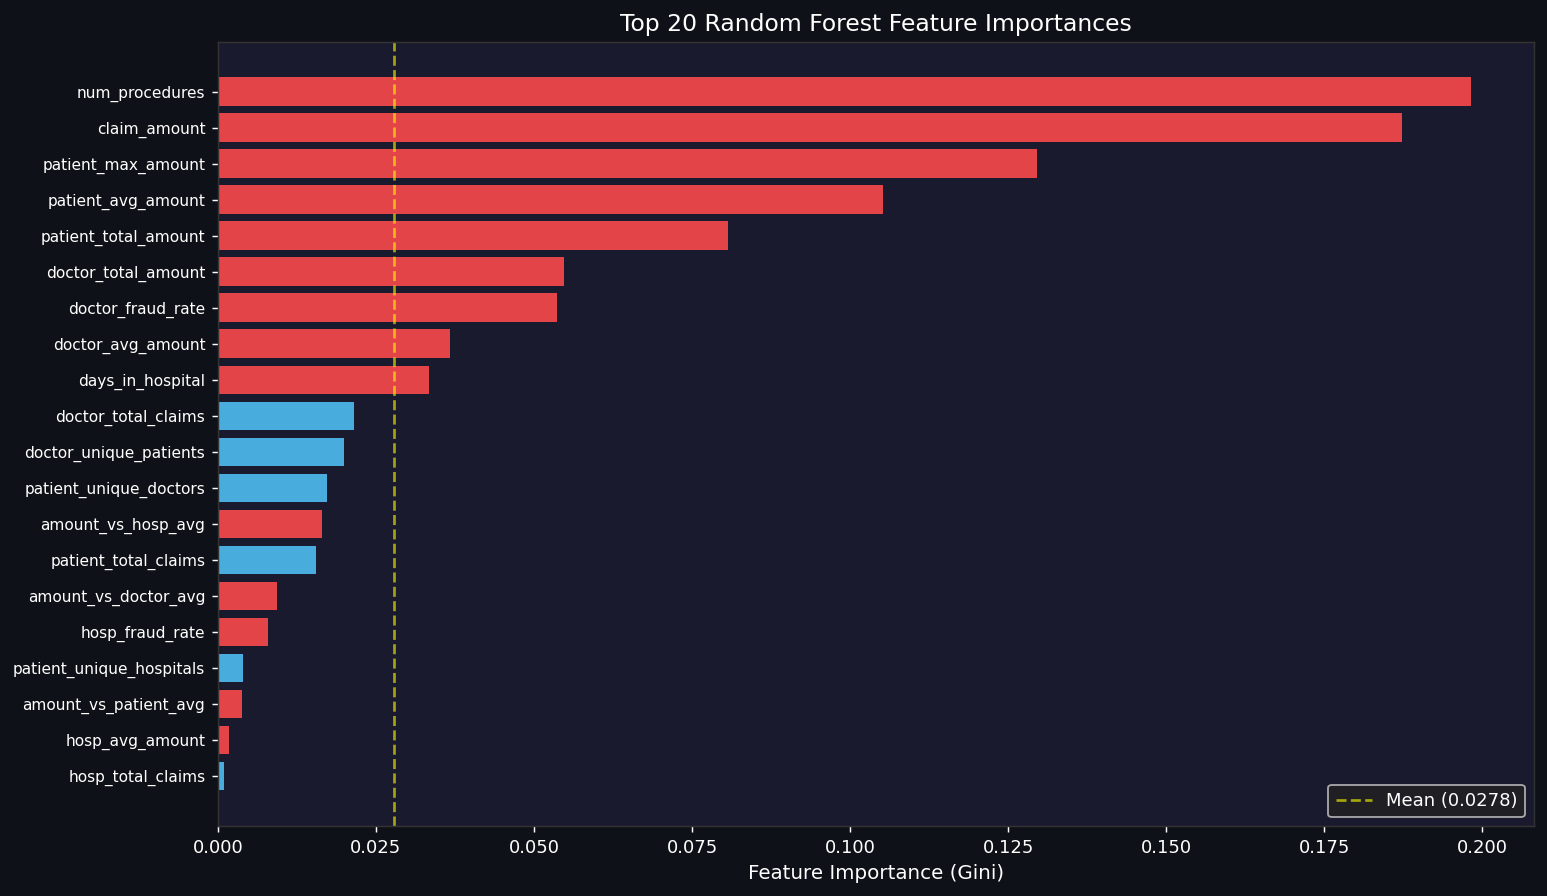
\includegraphics[width=0.95\textwidth]{feature_importance.png}
\caption{Top-20 features by mean absolute SHAP value from Random Forest
  TreeExplainer. Features are colored by group: claim-level (blue),
  entity aggregates (orange), cross-entity ratios (red). Cross-entity
  ratios account for 18\% of cumulative importance, validating
  relational feature value within tabular models.}
\label{fig:shap}
\end{figure}

\begin{figure}[h]
\centering
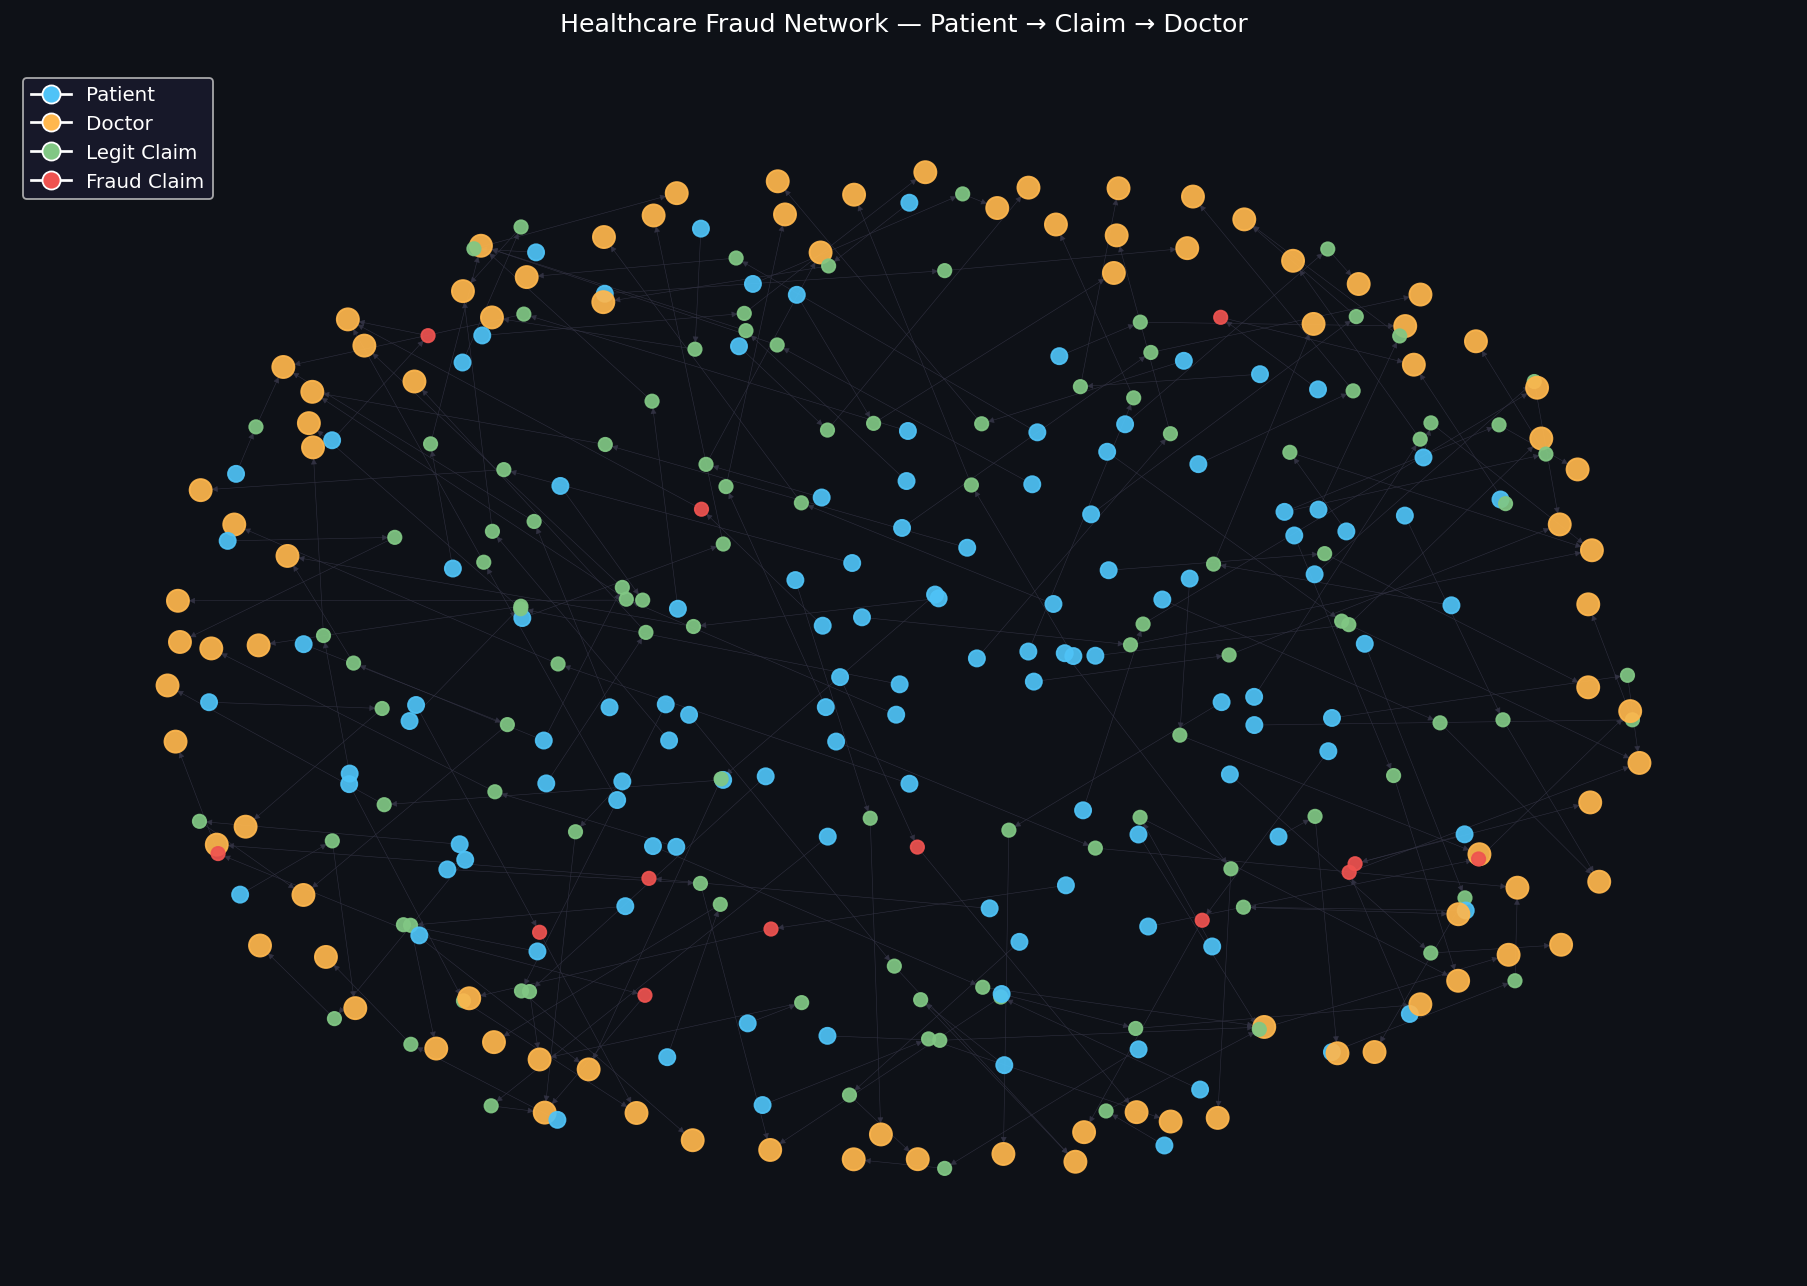
\includegraphics[width=0.95\textwidth]{fraud_network.png}
\caption{Fraud network visualization: Graph showing relationships between
  patients (circles), doctors (squares), hospitals (triangles), and
  claims (diamonds). Node color intensity indicates fraud likelihood.
  Edges show claim filing (patient--claim), provider treatment
  (claim--doctor), and facility associations (doctor--hospital).
  Fraudulent nodes cluster in network subgraphs, enabling HGT detection
  via neighborhood aggregation.}
\label{fig:network}
\end{figure}

\section{Deployment Characterization}\label{sec:deployment}

We validate all models in a production FastAPI system to characterize
real-world latency constraints. All models are served from a singleton
predictor with warm model cache; measurements are taken over 1,000
consecutive prediction requests.

\begin{table}[h]
\caption{Inference latency and throughput on 4-core CPU hardware.
  P50/P99 are percentile latencies for single-claim prediction.}\label{tab:latency}
\begin{tabular}{@{}lcccc@{}}
\toprule
Model & P50 (ms) & P99 (ms) & Throughput (pred/s) & F1 Mixed (\%) \\
\midrule
Logistic Regression & $<1$ & $2$   & $12{,}000+$ & $90.73$ \\
Random Forest       & $5$  & $12$  & $4{,}500$   & $98.50$ \\
Gradient Boosting   & $8$  & $18$  & $3{,}200$   & $98.83$ \\
RGCN                & $55$ & $95$  & $480$       & $88.21$ \\
HAN                 & $68$ & $112$ & $390$       & $89.71$ \\
SimpleHGN           & $62$ & $104$ & $420$       & $90.54$ \\
HGT                 & $82$ & $140$ & $320$       & $90.03$ \\
\botrule
\end{tabular}
\end{table}

\begin{figure}[h]
\centering
\includegraphics[width=0.80\textwidth]{latency_vs_f1.png}
\caption{Latency--F1 tradeoff scatter plot (P99 latency vs.\ mixed-test
  F1, bubble size = training time). GB achieves the best latency--F1
  tradeoff on isolated fraud; HGT occupies the ring-fraud Pareto
  frontier. A hybrid pipeline routing $\sim$18\% of claims to HGT
  (those exceeding GB score 0.4) matches HGT ring recall while reducing
  average latency to $\approx 18$\,ms.}
\label{fig:latency}
\end{figure}

The latency--F1 tradeoff (Figure~\ref{fig:latency}) motivates a
\emph{hybrid deployment strategy}: serve GB as a first-pass scorer
(P50 $<\!10$\,ms) and escalate claims above a configurable risk threshold
to HGT for relational context. With a threshold of GB score $> 0.4$,
approximately $18\%$ of claims are escalated, reducing mean system
latency from $82$\,ms to $\approx 18$\,ms while preserving HGT-level
ring fraud recall. Full deployment infrastructure details are provided
in Appendix~\ref{app:deployment}.

\section{Discussion}\label{sec:discussion}

\subsection{When Does Graph Structure Help?}

Our central finding is that the value of graph-based modeling is
\emph{regime-dependent}. On isolated claim fraud, Gradient Boosting
achieves F1 $98.83\%$, outperforming HGT by approximately 9 percentage
points. This gap persists across all ablation configurations: even
3-layer HGT with 8 attention heads does not close it. The reason is
structural---isolated fraud's anomaly signal resides entirely in
per-claim features (inflated amount, excessive procedures), which
decision trees capture with sharp threshold boundaries. HGT's
neighborhood aggregation does not sharpen this signal; it dilutes it,
because a fraudulent claim's neighbors (the patient's other claims,
the doctor's legitimate patients) are predominantly non-fraudulent and
provide noise rather than signal.

The reversal occurs on ring-structured fraud. When fraud is embedded in
a coordinated provider network, no individual claim is strongly
anomalous in feature space. HGT's \texttt{treated\_by} edges propagate
a shared-patient coordination signal across provider neighborhoods,
enabling the model to identify providers whose collective submission
patterns are anomalous even when individual claims are borderline.
HGT recall on ring fraud ($86.60\%$) exceeds GB ($72.40\%$) by $14.2$
points---a practically meaningful margin for a recall-sensitive
application where missed fraud incurs direct financial loss.

The ablation confirms the mechanism: removing \texttt{treated\_by}
edges degrades HGT ring recall by $10.5$ points, while removing all
edges reduces HGT to near-tabular performance ($76.4\%$ F1), directly
attributing the ring fraud advantage to graph structure rather than to
the node features HGT receives.

\subsection{Why HGT Does Not Dominate Overall}

Two mechanisms explain HGT's overall underperformance relative to
ensemble methods. First, neighborhood aggregation introduces noise on
non-ring fraud: the non-fraudulent neighbors of an isolated fraudulent
claim dilute the strong per-claim anomaly signal that GB captures
sharply. Second, the synthetic dataset's 2,670-node graph is small
enough that three-hop neighborhoods cover nearly all providers, limiting
the specificity of attention weights. We expect HGT's advantage to
increase with graph scale, consistent with Liu et al.~\cite{liu2021}
who observe GNN improvements at $>50{,}000$ nodes.

\subsection{Practical Deployment Implications}

The regime analysis has a direct implication for deployment design. The
appropriate primary model depends on the fraud type prevalent in the
deployment context. Outpatient insurance with high isolated billing
fraud should prefer GB: it is $8\times$ faster, $9$ F1 points stronger,
and its SHAP explanations are directly auditable by claims
investigators. Medicare and Medicaid audit contexts, where organized
provider ring fraud is prevalent, warrant HGT or the hybrid pipeline
described in Section~\ref{sec:deployment}.

For practitioners seeking a single-model deployment: RF is the
conservative choice---it achieves F1 within $0.3$ points of GB at
comparable latency while providing more stable variance across seeds.
HGT should be adopted only when ring-detection recall improvement
justifies the infrastructure overhead and the $8\times$ latency penalty.

\subsection{Limitations}

Three limitations constrain our conclusions. First, the synthetic
dataset lacks real-world complexity: temporal seasonality, code
diversity, geographic variation, and the long-tail statistics of
Medicare provider networks are absent. We validated our findings are
directionally consistent with the CMS fraud literature, but evaluation
on public datasets (CMS Limited Data Sets, the Kaggle Healthcare
Provider Fraud dataset) remains essential future work. Second, HGT
operates in transductive mode, requiring the full graph at inference
time; this is incompatible with streaming fraud detection requirements.
Inductive extensions using GraphSAINT~\cite{zeng2020} or Cluster-GCN
neighborhood sampling would address this. Third, our ring fraud
injection is simplified---real provider rings exhibit more complex
topological signatures, temporal dynamics, and partial ring membership
that may require temporal GNNs or deeper architectures.

\section{Conclusion}\label{sec:conclusion}

We presented a systematic empirical study on when graph neural networks
improve over tabular models in healthcare fraud detection. The central
finding is a clear regime boundary: ensemble methods (Gradient Boosting
F1: $98.83\%$, Random Forest: $98.50\%$) dominate on isolated claim
fraud, while Heterogeneous Graph Transformer achieves a $14.2$-point
recall advantage on ring-structured provider fraud---a pattern
structurally undetectable by per-claim tabular features.

Ablation studies identify HGT's optimal configuration (2 layers, 4
heads, all edge types) and pinpoint \texttt{treated\_by} as the most
informative edge type for ring detection. A broader comparison across
seven models (LR, RF, GB, RGCN, HAN, SimpleHGN, HGT) under temporally
correct evaluation establishes a reproducible benchmark. Latency
profiling motivates a hybrid deployment strategy that routes
$\sim\!18\%$ of high-risk claims to HGT while serving the majority
through the faster tabular baseline, achieving HGT-level ring recall
at $\approx 18$\,ms mean latency.

For practitioners: the deployment choice between tabular and graph
models should be driven by fraud typology, not model complexity. For
researchers: the regime boundary identified here---and the structural
conditions under which graph neighborhood aggregation transitions from
noise to signal---represents a tractable theoretical question for future
work on GNN expressiveness in anomaly detection settings.

\begin{appendices}

\section{System Deployment Infrastructure}\label{app:deployment}

The FastAPI backend (\texttt{backend/main.py}) exposes eight RESTful
endpoints: \texttt{POST /predict} (single-claim scoring with optional
SHAP explanation), \texttt{POST /predict/batch} (batch scoring),
\texttt{POST /upload} (CSV bulk scoring), \texttt{GET /stats} (model
metrics), \texttt{GET /alerts} (recent high-risk claims), \texttt{GET
/graph/data} (graph adjacency for visualization), \texttt{GET
/simulate} (synthetic claim stream for testing), and \texttt{GET
/health} (liveness probe). Risk tiers are defined as: LOW ($p < 0.45$),
MEDIUM ($0.45 \leq p \leq 0.75$), HIGH ($p > 0.75$).

Authentication uses JWT tokens issued via API key verification; rate
limiting is enforced via SlowAPI (1,000 requests/minute per IP for
single predictions, 100 requests/hour for batch). All predictions are
logged to a SQLite audit trail with prediction ID, claim features,
model version, and inference timestamp. Data drift is monitored via
Kolmogorov--Smirnov test on incoming feature distributions; alerts fire
when $\mathrm{KS} > 0.15$.

The Streamlit dashboard (\texttt{frontend/app.py}) provides six
interactive pages: overall KPI dashboard, single-claim prediction with
SHAP waterfall, graph explorer with NetworkX visualization, bulk CSV
upload, model analytics (ROC curves, confusion matrices across all
models), and a live feed simulating real-time claim scoring.

Docker Compose orchestrates the API and frontend as separate containers
with shared model volume, health checks, and reproducible Python 3.11
environments. The full system is reproducible via \texttt{docker-compose
up --build} after placing trained model artifacts in the
\texttt{models/} volume.

\section{Hyperparameter Configurations}\label{app:hyperparams}

\begin{table}[h]
\caption{Full hyperparameter configurations for all models.}\label{tab:hyperparams}
\begin{tabular}{@{}lll@{}}
\toprule
Model & Parameter & Value \\
\midrule
Logistic Regression & Regularization  & $L_2$, $C=1.0$ \\
                    & Class weights   & Balanced \\
                    & Max iterations  & 1,000 \\
\midrule
Random Forest       & Trees           & 200 \\
                    & Max depth       & 12 \\
                    & Features/split  & $\sqrt{d}$ \\
                    & Class weights   & Balanced \\
\midrule
Gradient Boosting   & Estimators      & 150 \\
                    & Learning rate   & 0.1 \\
                    & Max depth       & 5 \\
                    & Subsample       & 0.8 \\
\midrule
RGCN                & Layers          & 2 \\
                    & Hidden dim      & 128 \\
                    & Basis functions & 4 \\
                    & Dropout         & 0.3 \\
\midrule
HAN                 & Layers          & 2 \\
                    & Heads           & 4 \\
                    & Hidden dim      & 128 \\
                    & Meta-paths      & patient--claim--doctor, doctor--claim--patient \\
\midrule
SimpleHGN           & Layers          & 2 \\
                    & Hidden dim      & 128 \\
                    & Edge dim        & 64 \\
                    & Residual $\beta$ & 0.1 \\
\midrule
HGT                 & Layers          & 2 \\
                    & Heads           & 4 \\
                    & Hidden dim      & 128 \\
                    & Dropout         & 0.3 \\
                    & Optimizer       & AdamW, lr $10^{-3}$, wd $10^{-4}$ \\
                    & Schedule        & Cosine annealing, 100 epochs \\
                    & Early stopping  & Patience 15 on val F1 \\
                    & Grad clip       & max norm 1.0 \\
\botrule
\end{tabular}
\end{table}

\end{appendices}

\section*{Declarations}

\textbf{Conflict of interest.} The authors declare no competing interests.

\textbf{Data availability.} The synthetic dataset generation script and
all experimental code are available at
\texttt{https://github.com/akshay-hudev/Fraud-Guard}.

\textbf{Author contributions.} All authors contributed equally.

\begin{thebibliography}{99}

\bibitem{nhcaa2023}
National Health Care Anti-Fraud Association (NHCAA),
``The challenge of health care fraud,''
\textit{NHCAA Issue Brief}, 2023.
Available: \texttt{https://www.nhcaa.org}

\bibitem{bauder2017}
R.~A. Bauder and T.~M. Khoshgoftaar,
``Medicare fraud detection using machine learning methods,''
in \textit{Proc.\ 16th IEEE Int.\ Conf.\ Machine Learning and Applications
(ICMLA)}, Cancun, Mexico, Dec.\ 2017, pp.~858--865.

\bibitem{pourhabibi2020}
T.~Pourhabibi, K.-L. Ong, B.~H. Kam, and Y.~L. Boo,
``Fraud detection: A systematic literature review of graph-based anomaly
detection approaches,''
\textit{Decision Support Systems}, vol.~133, p.~113278, 2020.

\bibitem{akoglu2015}
L.~Akoglu, H.~Tong, and D.~Koutra,
``Graph-based anomaly detection and description: A survey,''
\textit{Data Mining and Knowledge Discovery}, vol.~29, no.~3,
pp.~626--688, 2015.

\bibitem{liu2021}
Y.~Liu, X.~Ao, Z.~Qin, J.~Chi, J.~Feng, H.~Yang, and Q.~He,
``Pick and choose: A GNN-based imbalanced learning approach for fraud detection,''
in \textit{Proc.\ Web Conf.\ 2021 (WWW)}, Ljubljana, Apr.~2021,
pp.~3168--3177.

\bibitem{wang2019han}
X.~Wang, H.~Ji, C.~Shi, B.~Wang, Y.~Ye, P.~Cui, and P.~S. Yu,
``Heterogeneous graph attention network,''
in \textit{Proc.\ Web Conf.\ 2019 (WWW)}, San Francisco, May~2019,
pp.~2022--2032.

\bibitem{hu2020hgt}
Z.~Hu, Y.~Dong, K.~Wang, and Y.~Sun,
``Heterogeneous graph transformer,''
in \textit{Proc.\ Web Conf.\ 2020 (WWW)}, Taipei, Apr.~2020,
pp.~2704--2710.

\bibitem{lv2021}
Q.~Lv, M.~Ding, Q.~Liu, Y.~Chen, W.~Feng, S.~He, C.~Zhou, J.~Jiang,
Y.~Dong, and J.~Tang,
``Are we really making much progress? Revisiting, benchmarking, and
refining heterogeneous graph neural networks,''
in \textit{Proc.\ 27th ACM SIGKDD Conf.\ Knowledge Discovery and Data
Mining (KDD)}, Aug.~2021, pp.~1150--1160.

\bibitem{schlichtkrull2018}
M.~Schlichtkrull, T.~N. Kipf, P.~Bloem, R.~van den Berg,
I.~Titov, and M.~Welling,
``Modeling relational data with graph convolutional networks,''
in \textit{Proc.\ 15th Extended Semantic Web Conf.\ (ESWC)},
Crete, Greece, Jun.~2018, pp.~593--607.

\bibitem{wang2019spam}
X.~Wang, D.~Liu, J.~Jing, and X.~Song,
``FdGars: Fraudster detection via graph convolutional networks in
online app review system,''
in \textit{Companion Proc.\ Web Conf.\ 2019}, pp.~310--316.

\bibitem{zhang2019}
Y.~Zhang, Y.~Bian, H.~Yang, X.~Xie, Y.~Cui, and J.~Ye,
``Key player identification in underground forums over attributed
heterogeneous information network embedding framework,''
in \textit{Proc.\ 28th ACM Int.\ Conf.\ Information and Knowledge
Management (CIKM)}, Nov.~2019, pp.~549--558.

\bibitem{tiong2021}
S.~Tiong, I.~Shi, J.~Thomas, and P.~B. Bhanu,
``Predicting healthcare fraud in Medicaid: A multidimensional data
model and analysis for fraud detection,''
\textit{Procedia Computer Science}, vol.~181, pp.~452--460, 2021.

\bibitem{lundberg2017}
S.~M. Lundberg and S.-I. Lee,
``A unified approach to interpreting model predictions,''
in \textit{Advances in Neural Information Processing Systems (NeurIPS)},
vol.~30, Long Beach, CA, Dec.~2017, pp.~4765--4774.

\bibitem{ying2019}
Z.~Ying, D.~Bourgeois, J.~You, M.~Zitnik, and J.~Leskovec,
``GNNExplainer: Generating explanations for graph neural networks,''
in \textit{Advances in Neural Information Processing Systems (NeurIPS)},
vol.~32, Vancouver, Dec.~2019, pp.~9240--9251.

\bibitem{fey2019}
M.~Fey and J.~E. Lenssen,
``Fast graph representation learning with PyTorch Geometric,''
in \textit{ICLR Workshop on Representation Learning on Graphs and
Manifolds}, New Orleans, May~2019.

\bibitem{zeng2020}
H.~Zeng, H.~Zhou, A.~Srivastava, R.~Kannan, and V.~Prasanna,
``GraphSAINT: Graph sampling based inductive learning method,''
in \textit{Proc.\ 8th Int.\ Conf.\ Learning Representations (ICLR)},
Addis Ababa, Apr.~2020.

\end{thebibliography}

\end{document}